\begin{figure}[htbp]
    \centering
    \resizebox{0.92\textwidth}{!}{%
    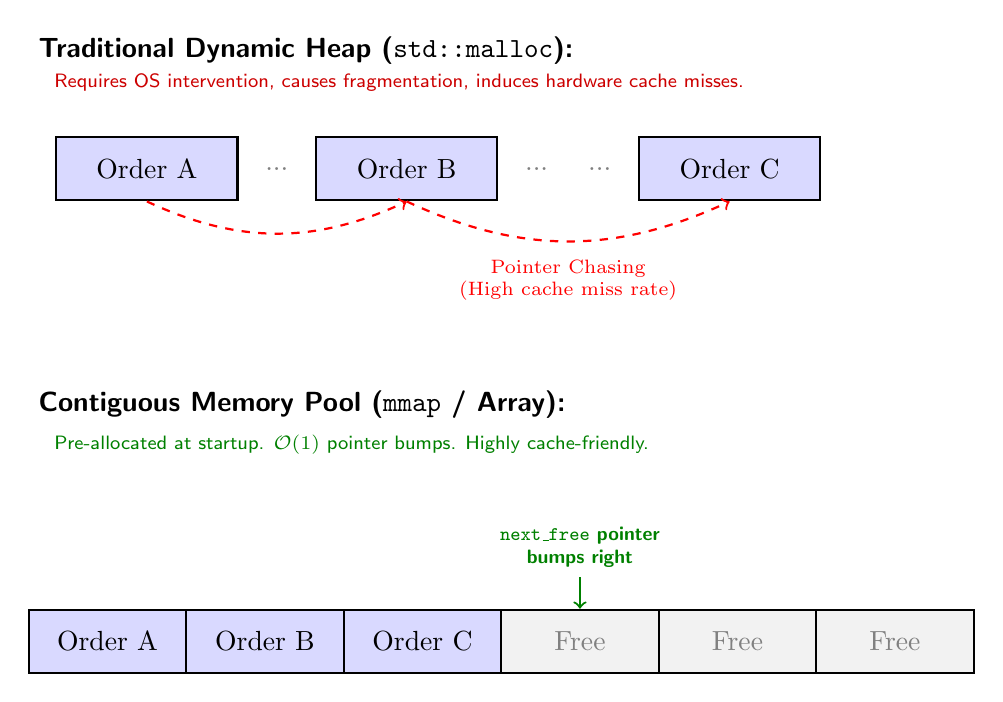
\begin{tikzpicture}[
        memory_block/.style={rectangle, draw=black, thick, minimum width=2.3cm, minimum height=0.8cm, align=center},
        used/.style={memory_block, fill=blue!15},
        free/.style={memory_block, fill=gray!10, text=gray},
        fragment/.style={rectangle, text=gray, minimum width=1.2cm, minimum height=0.8cm, align=center},
        arrow/.style={->, thick, >=stealth}
    ]

    % Top Section: Dynamic Heap Allocation
    \node[anchor=west, font=\sffamily\bfseries] at (0, 3.5) {Traditional Dynamic Heap (\texttt{std::malloc}):};
    \node[anchor=west, text=red!80!black, font=\sffamily\scriptsize, align=left] at (0.2, 3.1) {Requires OS intervention, causes fragmentation, induces hardware cache misses.};

    % Fragmented Blocks manually positioned
    \node[used] (m1) at (1.5, 2.0) {Order A};
    \node[fragment] (gap1) at (3.15, 2.0) {...};
    \node[used] (m2) at (4.8, 2.0) {Order B};
    \node[fragment] (gap2) at (6.85, 2.0) {... \quad ...};
    \node[used] (m3) at (8.9, 2.0) {Order C};

    % Memory pointer randomly jumping (Pointer Chasing)
    \draw[->, dashed, color=red, thick] (m1.south) to[out=-25, in=205] (m2.south);
    \draw[->, dashed, color=red, thick] (m2.south) to[out=-25, in=205] node[below, font=\scriptsize, align=center, pos=0.5, yshift=-0.1cm] {Pointer Chasing\\(High cache miss rate)} (m3.south);

    % Bottom Section: Memory Pool
    \node[anchor=west, font=\sffamily\bfseries] at (0, -1.0) {Contiguous Memory Pool (\texttt{mmap} / Array):};
    \node[anchor=west, text=green!50!black, font=\sffamily\scriptsize, align=left] at (0.2, -1.5) {Pre-allocated at startup. $\mathcal{O}(1)$ pointer bumps. Highly cache-friendly.};

    % Contiguous Blocks manually positioned (width=2.0cm each)
    \node[used, minimum width=2.0cm] (p1) at (1.0, -4.0) {Order A};
    \node[used, minimum width=2.0cm] (p2) at (3.0, -4.0) {Order B};
    \node[used, minimum width=2.0cm] (p3) at (5.0, -4.0) {Order C};
    \node[free, minimum width=2.0cm] (p4) at (7.0, -4.0) {Free};
    \node[free, minimum width=2.0cm] (p5) at (9.0, -4.0) {Free};
    \node[free, minimum width=2.0cm] (p6) at (11.0, -4.0) {Free};

    % Contiguous borders adjustment (overlapping lines manually fixed by drawing them tight, but TikZ standard nodes look fine adjacent)

    % Free pointer bump
    \draw[<-, thick, color=green!50!black] (p4.north) -- +(0, 0.4) node[above, font=\sffamily\bfseries\scriptsize, align=center] {\texttt{next\_free} pointer\\bumps right};

    \end{tikzpicture}%
    }
    \caption{Visual comparison of traditional heap allocation versus a Memory Pool. Dynamic allocations mathematically fragment across the heap as orders are rapidly added and deleted, forcing the CPU to fetch disjointed cache lines ("pointer chasing"). A Memory Pool allocates one massive contiguous block upfront, ensuring subsequent active object fetches naturally stream into the L1 hardware cache.}
    \label{fig:memory_pool}
\end{figure}
